\documentclass[final]{beamer}
\usetheme{SD}
\usepackage[orientation=landscape,size=custom,width=160,height=90,scale=2.4,debug]{beamerposter}
%\usepackage[absolute,overlay]{textpos}
%\setlength{\TPHorizModule}{1cm}
%\setlength{\TPVertModule}{1cm}
\usepackage{graphicx}
\usepackage{caption}
\usepackage{subcaption}
\usepackage{wrapfig}

\title{Scientific Computing Interest Group}
\author{Sean Davis, Jeff Shilling, and Carl McCabe}
\date{January 14, 2014}
\footer{}

\begin{document}
\begin{frame}[t]
  \begin{columns}[t]

% FIRST column
    \begin{column}{0.3\linewidth}
      \begin{block}{Intramural NCI and Scientific Computing}
The NCI Intramural Research Program (IRP) is large and diverse.  Despite this research diversity, data and computation across the IRP are critical, ubiquitous, and potentially unifying.  The Scientific Computing Interest Group is a grass-roots effort to enhance the environment for successful computational and data science in the IRP.
      \end{block}
      \begin{block}{Research Software Development}
\small{Software development and publication is an increasingly important component in the NCI IRP mission. Recently developed and evolving guidelines are available as a set of Frequently Asked Questions.}
{\tiny
\begin{itemize}
\item{Am I required to make software code I have developed available upon request?}
\item{Am I required to actively disseminate code I have developed?}
\item{How do I determine if NCI/NIH has ownership over the software code?}
\item{What are my options for protecting works I have largely contributed to or developed?}
\item{How do I release software source code to the public?}
\item{Are there guidelines and/or restrictions to using social media tools for collaborating with the public? (e.g. Github)}
\item{Must I obtain certain NCI/NIH permissions before releasing software code to the public?}
\item{Is there a specific time frame by which the code must be released to the public?}
\item{How thoroughly should I document my code?}
\item{What are the advantages of releasing software code as free open source?}
\item{Should I license my code?  If so, why?}
\item{How do I choose a license under which to release my code?}
\item{Should I write a custom license under which to release my code?}
\item{How should I acknowledge NIH as the source funding the research software that I develop?}
\item{Should I develop my software for desktop execution or as a web application?}
\item{Can my software's user interface contain NCI or NIH logos?}
\item{Am I expected to provide technical support in perpetuity?}
\item{How can I retain control over open source software?}
\item{Can I put stipulations on who can access and use my software?}
\item{How can I require acknowledgement from people publishing research based on my software or software derived from it?}
\item{Does NCI or NIH have any requirements related to beta testing my software?}
\item{What QA/QC steps are required of me before releasing my software? }
\item{My software may possibly be used in medical practice or clinical settings.  What additional steps should I take before release?}
\item{How do I vet my software against security flaws?}
\item{How can I reference my software in a publication so that readers may access it?}
\item{After my software has been released, how can I notify users of updates?  And, what responsibility do I have for maintaining or updating the software?}
\end{itemize}
}
\end{block}
\end{column}
% BEGIN SECOND column
    \begin{column}{0.3\linewidth}
      \begin{block}{Goals of the Interest Group}
        \begin{itemize}
        \item{Provide a general forum for discussion of computational issues}
        \item{Share best practices for Reproducible Research}
        \item{Share computational tools and methods}
        \item{Enhance knowledge management and collaboration related to data and computation}
        \item{Collect input about IT infrastructure needs in support of science}
        \item{Communicate IT and computational needs to IRP senior leadership}
        \item{Interface with IT groups both within and outside the NCI}
        \end{itemize}
      \end{block}
      \begin{block}{Speaker Series}
        \begin{figure}
          \centering
          \begin{subfigure}{.45\textwidth}
            \centering
            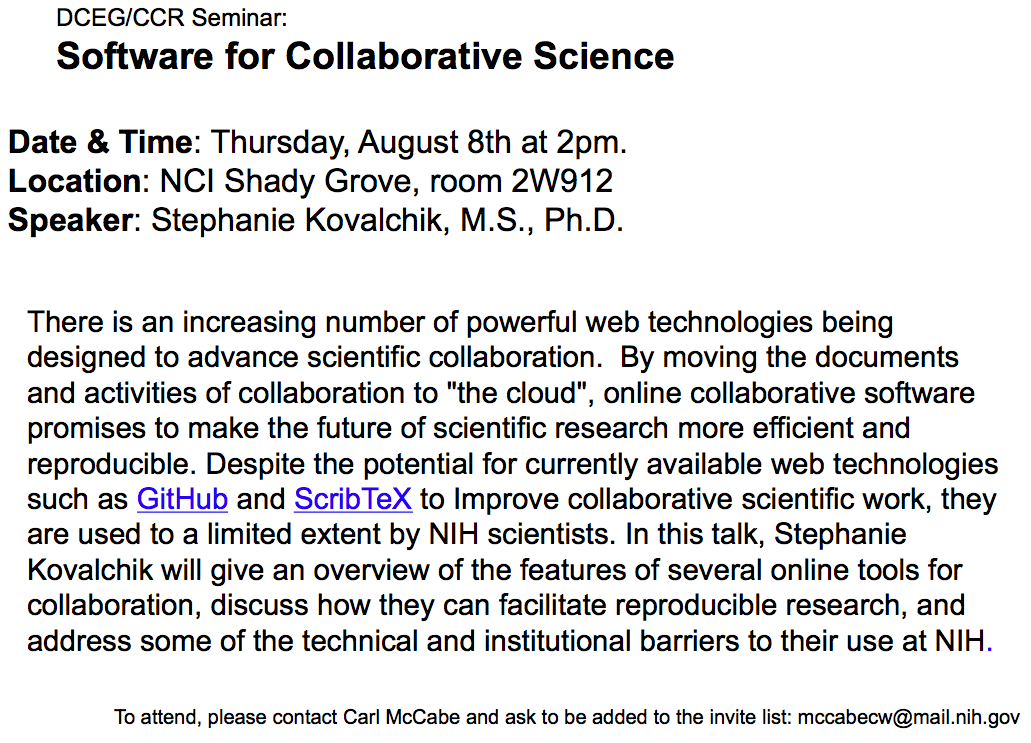
\includegraphics[width=1\linewidth]{collabSoftwareTools}
            \label{fig:sub1}
          \end{subfigure}
          \begin{subfigure}{.45\textwidth}
            \centering
            
\includegraphics[width=1\linewidth]{helixOverview}
            \label{fig:sub2}
          \end{subfigure}
          \label{fig:test}
        \end{figure}
      {\small
      \begin{itemize}
      \item{Potential speaker topics}
        \begin{itemize}
        \item{Scientific Workflow Management with \textit{make-like} Tools}
        \item{Introduction to Relational Databases}
        \item{Reporting Tools for the R Statistics Package}
        \item{Tools for Scientific Collaboration in a Data-centric World}
        \end{itemize}
      \end{itemize}
      }
      \end{block}

    \end{column}

% BEGIN THIRD column
    \begin{column}{0.3\linewidth}
      \begin{block}{High Performance Computing}
        \begin{figure}
          \begin{center}
            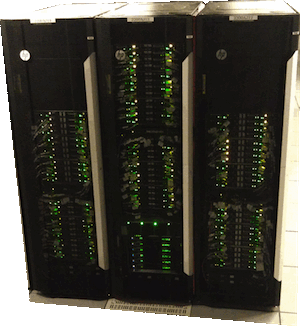
\includegraphics[width=0.4\linewidth]{20130102-LCP-nodes}
          \end{center}
          \label{fig:biowulf}
        \end{figure}
{\small
The NCI IRP supports several high performance compute clusters, including those supported by the CCR and DCEG.
        \begin{itemize}
          \item{The CCR Compute Resource}
            \begin{itemize}
            \item{Priority compute nodes on the NIH Biowulf system}
            \item{Hardware: 128 nodes x 32 cores with either 64GB or 128GB RAM}
            \item{Storage: Shares storage with the Biowulf system}
            \item{No cost (except Helix account) to CCR investigators to use}
            \end{itemize}
          \item{Compute Cluster at DCEG (CCAD)}
            \begin{itemize}
            \item{Hardware: 43 x 16 cores, 128GB RAM}
            \end{itemize}
        \end{itemize}
}
            
      \end{block}
      \begin{block}{Getting Involved}
        \begin{itemize}
          \item{Volunteer to give a talk}
          \item{Suggest topics for the Speaker Series}
          \item{Share your ideas with us about how to improve the Interest Group}
          \item{Email us with questions or comments:}
            \begin{itemize}
              \item{sdavis2@mail.nih.gov}
              \item{shillingj@mail.nih.gov}
              \item{carl.mccabe@nih.gov}
                
            \end{itemize}
          \end{itemize}
        \end{block}
    \end{column}
    \end{columns}
  \end{frame}
\end{document}
